\documentclass[10pt,a4paper]{article}
\usepackage[a4paper,top=3.3cm,bottom=2.1cm,left=1.5cm,right=1.5cm,headheight=42pt,headsep=10pt,footskip=24pt]{geometry}
\usepackage[T1]{fontenc}
\usepackage{amsmath,amssymb}
\usepackage{xcolor}
\usepackage{tikz}
\usetikzlibrary{arrows.meta,calc,patterns}
\usepackage{fancyhdr}
\usepackage{lastpage}
\usepackage{tabularx}
\usepackage{array}
\usepackage{multicol}
\usepackage{needspace}
\usepackage{pifont}

\definecolor{spsblue}{RGB}{20,50,120}
\definecolor{spsgrey}{RGB}{110,110,110}
\setlength{\columnsep}{0.8cm}
\setlength{\columnseprule}{0.4pt}

% ---------- header / footer ----------
\pagestyle{fancy}
\fancyhf{}
\renewcommand{\headrulewidth}{0.9pt}
\renewcommand{\footrulewidth}{0.5pt}
\fancyhead[C]{%
  {\Large\bfseries\color{spsblue}SAGAR PUBLIC SCHOOL}\\[2pt]
  {\small\bfseries Integrated Programme \quad$\bullet$\quad Topic: \sheettopic}}
\fancyfoot[L]{\footnotesize Sagar Public School}
\fancyfoot[C]{\footnotesize Integrated Programme \,|\, Gravitation -- Practice Sheet \sheetno}
\fancyfoot[R]{\footnotesize Page \thepage\ of \pageref{LastPage}}
\setlength{\parindent}{0pt}
\setlength{\parskip}{0pt}
\renewcommand{\arraystretch}{1.2}

% ---------- question machinery ----------
\newcounter{qn}
\newcommand{\cursrc}{}
\newenvironment{question}[1]{%
  \par\vspace{6pt}\def\cursrc{#1}%
  \begin{minipage}{\linewidth}\refstepcounter{qn}\textbf{Q.\theqn}\quad\ignorespaces}%
 {\par\vspace{1pt}\hfill{\tiny\color{spsgrey}[\cursrc]}\end{minipage}\par}
\newcommand{\secthead}[1]{\par\vspace{8pt}\noindent\begin{minipage}{\linewidth}{\normalsize\bfseries\color{spsblue}#1}\par\vspace{1pt}\hrule height 0.6pt\end{minipage}\par\nobreak}

\newcommand{\labA}{A}\newcommand{\labB}{B}\newcommand{\labC}{C}\newcommand{\labD}{D}
\newcommand{\numlabels}{\renewcommand{\labA}{1}\renewcommand{\labB}{2}\renewcommand{\labC}{3}\renewcommand{\labD}{4}}
\newcommand{\letterlabels}{\renewcommand{\labA}{A}\renewcommand{\labB}{B}\renewcommand{\labC}{C}\renewcommand{\labD}{D}}
\newcommand{\optsfour}[4]{\par\vspace{2pt}\hspace*{1em}\begin{tabularx}{\dimexpr\linewidth-1em\relax}{*{4}{>{\raggedright\arraybackslash}X}}
 (\labA) #1 & (\labB) #2 & (\labC) #3 & (\labD) #4\end{tabularx}\par}
\newcommand{\optstwo}[4]{\par\vspace{2pt}\hspace*{1em}\begin{tabularx}{\dimexpr\linewidth-1em\relax}{*{2}{>{\raggedright\arraybackslash}X}}
 (\labA) #1 & (\labB) #2 \\ (\labC) #3 & (\labD) #4\end{tabularx}\par}
\newcommand{\optsone}[4]{\par\vspace{2pt}\begin{list}{}{\setlength{\leftmargin}{2.3em}\setlength{\labelwidth}{2em}\setlength{\itemsep}{0pt}\setlength{\topsep}{0pt}\setlength{\parsep}{0pt}}
 \item[(\labA)] #1 \item[(\labB)] #2 \item[(\labC)] #3 \item[(\labD)] #4 \end{list}\par}

\tikzset{fig/.style={line width=0.8pt,>={Stealth[length=2mm]}}}

% Motion Ex-I Q.16 : one square panel / four panels
\newcommand{\sqpanel}[6]{\begin{tikzpicture}[fig,line width=0.7pt]
 \node[left] at (-0.1,0.9) {(#1)};
 \draw (0,0) rectangle (1.8,1.8);
 \foreach \p in {(0.55,1.3),(1.25,1.3),(0.9,0.9),(0.55,0.45),(1.25,0.45)} \fill \p circle (3pt);
 \node[anchor=north west,inner sep=1pt] at (0,1.8) {\scriptsize #2};
 \node[anchor=north east,inner sep=1pt] at (1.8,1.8) {\scriptsize #3};
 \node[anchor=south west,inner sep=1pt] at (0,0) {\scriptsize #4};
 \node[anchor=south east,inner sep=1pt] at (1.8,0) {\scriptsize #5};
 \node[anchor=west,inner sep=2pt] at (0.95,0.92) {\scriptsize #6};
\end{tikzpicture}}
\newcommand{\figSquares}{\sqpanel{A}{5M}{3M}{M}{5M}{M}\hspace{0.5cm}\sqpanel{B}{2M}{3M}{M}{2M}{M}\\[6pt]
 \sqpanel{C}{5M}{3M}{M}{5M}{2M}\hspace{0.5cm}\sqpanel{D}{2M}{3M}{M}{2M}{2M}}

% JEE Main 2026 22 Jan Morning : four masses at corners
\newcommand{\figSquare}{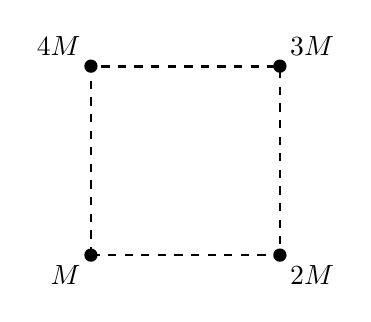
\begin{tikzpicture}[fig]
 \draw[dashed,line width=1pt] (0,0) rectangle (2.4,2.4);
 \foreach \p in {(0,0),(2.4,0),(0,2.4),(2.4,2.4)} \fill \p circle (2.4pt);
 \node[above left] at (0,2.4) {$4M$}; \node[above right] at (2.4,2.4) {$3M$};
 \node[below left] at (0,0) {$M$}; \node[below right] at (2.4,0) {$2M$};
\end{tikzpicture}}

% Motion Ex-I Q.22 : energy versus orbit radius
\newcommand{\figEnergy}{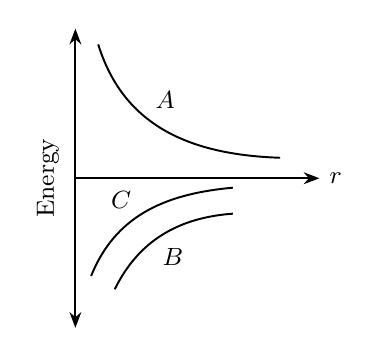
\begin{tikzpicture}[fig,line width=0.7pt]
 \draw[<->] (0,-1.9)--(0,1.9); \node[rotate=90] at (-0.35,0) {\small Energy};
 \draw[->] (0,0)--(3.1,0) node[right] {\small $r$};
 \draw (0.29,1.7) .. controls (0.6,0.7) and (1.4,0.3) .. (2.6,0.26); \node at (1.14,1.0) {\small $A$};
 \draw (0.2,-1.24) .. controls (0.5,-0.5) and (1.1,-0.2) .. (2.0,-0.12); \node at (0.58,-0.28) {\small $C$};
 \draw (0.5,-1.41) .. controls (0.8,-0.8) and (1.3,-0.5) .. (2.0,-0.45); \node at (1.24,-1.0) {\small $B$};
\end{tikzpicture}}

% Motion Ex-III Q.9 : two satellites on a collision course
\newcommand{\figOrbit}{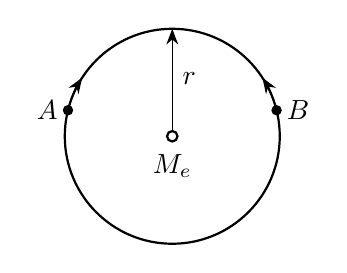
\begin{tikzpicture}[fig,scale=1.05]
 \draw (0,0) circle (1.3);
 \draw[->,line width=0.5pt] (0,0) -- (0,1.3); \node[right] at (0,0.7) {$r$};
 \draw[fill=white] (0,0) circle (1.8pt); \node[below] at (0,-0.1) {$M_e$};
 \fill (166:1.3) circle (1.8pt); \node[left] at (166:1.3) {$A$};
 \fill (14:1.3) circle (1.8pt); \node[right] at (14:1.3) {$B$};
 \draw[->,line width=0.5pt] (166:1.3) arc (166:147:1.3);
 \draw[->,line width=0.5pt] (14:1.3) arc (14:33:1.3);
\end{tikzpicture}}

% Motion Ex-III Q.15 : sphere with spherical hole
\newcommand{\figHole}{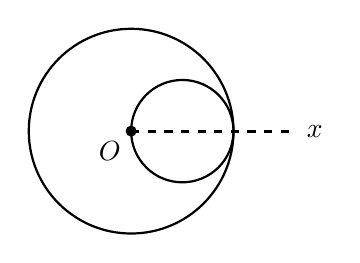
\begin{tikzpicture}[fig]
 \draw (0,0) circle (1.3); \draw (0.65,0) circle (0.65);
 \fill (0,0) circle (2pt); \node[below left] at (0,0) {$O$};
 \draw[dashed,line width=1pt] (0,0)--(2.1,0); \node[right] at (2.1,0) {$x$};
\end{tikzpicture}}

% Motion Ex-IV Q.3 : infinite rod with lambda(x) = lambda / x
\newcommand{\figInfRod}{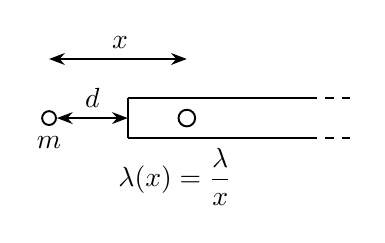
\begin{tikzpicture}[fig,line width=0.7pt]
 \draw (0,0) circle (2.5pt); \node[below] at (0,-0.1) {$m$};
 \draw[<->] (0.1,0)--(1.0,0); \node[above] at (0.55,0) {$d$};
 \draw (1.0,-0.25)--(1.0,0.25); \draw (1.0,0.25)--(3.3,0.25); \draw (1.0,-0.25)--(3.3,-0.25);
 \draw[dashed] (3.3,0.25)--(3.9,0.25); \draw[dashed] (3.3,-0.25)--(3.9,-0.25);
 \draw[fill=white] (1.75,0) circle (3pt);
 \draw[<->] (0,0.75)--(1.75,0.75); \node[above] at (0.9,0.75) {$x$};
 \node at (1.6,-0.75) {$\lambda(x)=\dfrac{\lambda}{x}$};
\end{tikzpicture}}

% Nucleus JM Q.10 (JEE Main 2017) : g versus d
\newcommand{\gpanel}[2]{\begin{tikzpicture}[fig,line width=0.7pt,scale=0.85]
 \draw[->] (0,0)--(2.4,0) node[right] {\scriptsize $d$}; \draw[->] (0,0)--(0,1.8) node[above] {\scriptsize $g$};
 \node[below left] at (0,0) {\scriptsize $O$}; \node[left] at (-0.25,0.9) {(#1)};
 #2
\end{tikzpicture}}
\newcommand{\figGraphs}{%
 \gpanel{1}{\draw (0,0) .. controls (0.9,0) and (1.5,0.3) .. (1.95,1.6);}\hspace{0.6cm}
 \gpanel{2}{\draw (0,0) .. controls (0.6,0.05) and (0.95,0.5) .. (1.1,1.5) .. controls (1.25,0.5) and (1.7,0.08) .. (2.2,0.02);
  \draw[dotted] (1.1,0)--(1.1,1.5); \node[below] at (1.1,0) {\scriptsize $R$};}\\[6pt]
 \gpanel{3}{\draw (0,0) .. controls (0.6,0.05) and (0.95,0.5) .. (1.1,1.5) -- (1.85,0);
  \draw[dotted] (1.1,0)--(1.1,1.5); \node[below] at (1.1,0) {\scriptsize $R$};}\hspace{0.6cm}
 \gpanel{4}{\draw (0,0)--(1.1,1.5) .. controls (1.25,0.5) and (1.7,0.08) .. (2.2,0.02);
  \draw[dotted] (1.1,0)--(1.1,1.5); \node[below] at (1.1,0) {\scriptsize $R$};}}

% Nucleus JM Q.8 (JEE Main 2015) : sphere with cavity
\newcommand{\figCavityHatch}{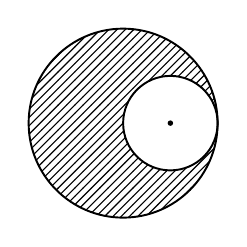
\begin{tikzpicture}[fig,line width=0.7pt]
 \path[pattern=north east lines,even odd rule] (0,0) circle (1.2) (0.6,0) circle (0.6);
 \draw (0,0) circle (1.2); \draw (0.6,0) circle (0.6); \fill (0.6,0) circle (1pt);
\end{tikzpicture}}

% Nucleus JM Q.35 (JEE Main 2021) : two satellites
\newcommand{\figTwoSat}{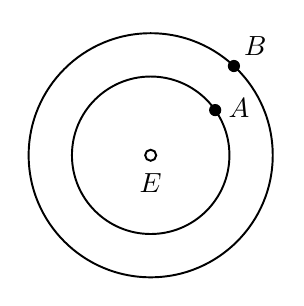
\begin{tikzpicture}[fig,line width=0.7pt]
 \draw (0,0) circle (1.0); \draw (0,0) circle (1.55);
 \draw[fill=white] (0,0) circle (2pt); \node[below] at (0,-0.1) {$E$};
 \fill (35:1.0) circle (2.2pt); \node[right] at (35:1.05) {$A$};
 \fill (47:1.55) circle (2.2pt); \node[above right] at (47:1.55) {$B$};
\end{tikzpicture}}

% JEE Main 2025 22 Jan Morning : sphere with spherical part removed
\newcommand{\figHoleP}{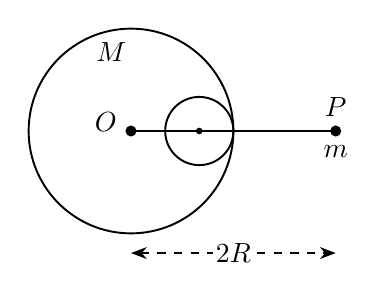
\begin{tikzpicture}[fig,line width=0.7pt]
 \draw (0,0) circle (1.3); \draw (0.867,0) circle (0.433);
 \fill (0,0) circle (2pt); \node[left] at (-0.05,0.12) {$O$};
 \fill (0.867,0) circle (1.2pt);
 \draw (0,0)--(2.6,0); \fill (2.6,0) circle (2pt);
 \node[above] at (2.6,0.05) {$P$}; \node[below] at (2.6,-0.05) {$m$};
 \node at (-0.25,1.0) {$M$};
 \draw[<->,dashed] (0,-1.55)--(2.6,-1.55); \node[fill=white,inner sep=1pt] at (1.3,-1.55) {$2R$};
\end{tikzpicture}}

% ---------- title block, answer key items, self assessment ----------
\newcommand{\titleblock}[2]{%
 \begin{center}
  {\Large\bfseries PRACTICE SHEET -- \sheetno}\\[2pt]
  {\normalsize\bfseries #1}
 \end{center}
 \vspace{1pt}
 \noindent\begin{tabularx}{\linewidth}{|X|X|X|}\hline
  Name: \hrulefill & Class / Section: \hrulefill & Date: \hrulefill \\ \hline
  \textbf{Time Allowed: 60 Mins} & \textbf{Total Questions: #2} & Roll No.: \hrulefill \\ \hline
 \end{tabularx}
 \par\vspace{4pt}}
\newcommand{\keyitem}[3]{\par\noindent\begin{minipage}{\linewidth}\textbf{#1.} {\scriptsize\color{spsgrey}[#2]}\ \ #3\end{minipage}\par\vspace{5pt}}

\newcommand{\selfassess}{%
 \clearpage
 \begin{center}{\Large\bfseries SELF ASSESSMENT -- Practice Sheet \sheetno}\end{center}
 \noindent\textit{Fill this in after checking your answers with the Answer Key.}\par\vspace{6pt}
 \noindent\begin{tabularx}{\linewidth}{|X|X|}\hline
  \textbf{Time Allowed:} 60 Mins & \textbf{Time Taken:} \rule{2.2cm}{0.4pt} Mins \\ \hline
  Start time: \rule{2cm}{0.4pt} & End time: \rule{2cm}{0.4pt} \\ \hline
  \multicolumn{2}{|l|}{Finished within the allowed time?\quad $\square$ Yes \quad $\square$ No \quad (extra / saved time: \rule{1.6cm}{0.4pt} Mins)} \\ \hline
 \end{tabularx}
 \par\vspace{8pt}
 \noindent\begin{tabularx}{\linewidth}{|>{\centering\arraybackslash}X|>{\centering\arraybackslash}X|>{\centering\arraybackslash}X|>{\centering\arraybackslash}X|>{\centering\arraybackslash}X|}\hline
  \textbf{Total} & \textbf{Attempted} & \textbf{Correct} & \textbf{Incorrect} & \textbf{Not attempted} \\ \hline
  15 & \rule[-4pt]{0pt}{18pt} & & & \\ \hline
 \end{tabularx}
 \par\vspace{3pt}
 \noindent Score (Correct $/$ 15): \rule{1.8cm}{0.4pt} \qquad Percentage: \rule{1.8cm}{0.4pt}\,\%
 \par\vspace{8pt}
 \noindent\textbf{Question-wise tracker} \hfill {\footnotesize write \ding{51} (correct), \ding{55} (incorrect) or $-$ (not attempted)}\par\vspace{3pt}
 \noindent\begin{tabularx}{\linewidth}{|*{8}{>{\centering\arraybackslash}X|}}\hline
  1&2&3&4&5&6&7&8\\ \hline \rule[-5pt]{0pt}{18pt}&&&&&&&\\ \hline
  9&10&11&12&13&14&15& \\ \hline \rule[-5pt]{0pt}{18pt}&&&&&&&\\ \hline
 \end{tabularx}
 \par\vspace{8pt}
 \noindent\textbf{Reason for the incorrect / unattempted questions} (write question numbers)\par\vspace{2pt}
 \noindent\begin{tabularx}{\linewidth}{|X|X|}\hline
  Concept not clear: \hrulefill & Formula forgotten: \hrulefill \\ \hline
  Calculation / silly mistake: \hrulefill & Ran out of time: \hrulefill \\ \hline
 \end{tabularx}
 \par\vspace{8pt}
 \noindent\textbf{Personal feedback guide (tick the band that matches your score)}\par\vspace{2pt}
 \noindent\begin{tabularx}{\linewidth}{|c|c|X|}\hline
  & \textbf{Correct} & \textbf{What to do next} \\ \hline
  $\square$ & 14--15 & Excellent. Concept and speed are both strong. Move to harder JEE-level problems and keep revising formulae once a week. \\ \hline
  $\square$ & 11--13 & Good. Re-do every incorrect question without looking at the solution, then note the formula or idea you missed. \\ \hline
  $\square$ & 7--10 & Fair. Revise the theory of escape speed, orbital speed, energies of a satellite and Kepler's laws, then re-attempt this sheet after 3 days. \\ \hline
  $\square$ & 0--6 & Needs attention. Re-read the chapter notes and solved examples first, then attempt this sheet again in two parts of 30 mins. \\ \hline
 \end{tabularx}
 \par\vspace{8pt}
 \noindent\textbf{My personal feedback / action plan:}\par\vspace{4pt}
 \noindent\rule{\linewidth}{0.4pt}\par\vspace{9pt}\noindent\rule{\linewidth}{0.4pt}\par\vspace{9pt}\noindent\rule{\linewidth}{0.4pt}\par\vspace{9pt}\noindent\rule{\linewidth}{0.4pt}
 \par\vspace{10pt}
 \noindent\textbf{Teacher's remarks:}\par\vspace{4pt}
 \noindent\rule{\linewidth}{0.4pt}\par\vspace{9pt}\noindent\rule{\linewidth}{0.4pt}
 \par\vspace{14pt}
 \noindent Student's signature: \rule{4cm}{0.4pt} \hfill Teacher's signature: \rule{4cm}{0.4pt}}
\newcommand{\sheetno}{3}
\newcommand{\sheettopic}{Gravitation -- Level 3 (Advanced)}
\begin{document}
\titleblock{Gravitation -- Level 3 (Advanced): Practice Sheet 3 of 3}{15}
\noindent\textbf{Instructions:} Attempt all 15 questions. Questions with options have only one correct option; the others need full working. Sections: A -- Acceleration due to Gravity, B -- Gravitational Potential and Potential Energy, C -- Motion of Satellite, D -- Newton's Law, Gravitational Field and Kepler's Laws. Time Allowed: 60 Mins.

\begin{multicols}{2}
\numlabels
\secthead{Section A -- Acceleration due to Gravity}

\begin{question}{Nucleus, JM Q.28 \; [JEE Main-2020]}
The acceleration due to gravity on the earth's surface at the poles is $g$ and angular velocity of the earth about the axis passing through the pole is $\omega$. An object is weighed at the equator and at a height $h$ above the poles by using a spring balance. If the weights are found to be same, then $h$ is: ($h\ll R$, where $R$ is the radius of the earth)
\optstwo{$\dfrac{R^2\omega^2}{g}$}{$\dfrac{R^2\omega^2}{4g}$}{$\dfrac{R^2\omega^2}{2g}$}{$\dfrac{R^2\omega^2}{8g}$}
\end{question}

\begin{question}{Nucleus, JM Q.10 \; [JEE Main 2017]}
The variation of acceleration due to gravity $g$ with distance $d$ from centre of the earth is best represented by ($R$ = Earth's radius):
\begin{center}\figGraphs\end{center}
\end{question}

\begin{question}{Motion, Ex-III Q.8}
Calculate the distance from the surface of the earth at which above and below the surface acceleration due to gravity is the same.
\end{question}

\begin{question}{Nucleus, S-1 Q.6}
The Earth may be regarded as a spherically shaped uniform core of density $\rho_1$ and radius $R/2$ surrounded by a uniform shell of thickness $R/2$ and density $\rho_2$. Find the ratio $\dfrac{\rho_1}{\rho_2}$ if the value of acceleration due to gravity is the same at surface as at depth $R/2$ from the surface.
\end{question}

\secthead{Section B -- Gravitational Potential and Potential Energy}

\begin{question}{Motion, Ex-III Q.3}
An object is projected vertically upward from the surface of the earth of mass $M$ with a velocity such that the maximum height reached is eight times the radius $R$ of the earth. Calculate:\\
(i) the initial speed of projection\\
(ii) the speed at half the maximum height.
\end{question}

\begin{question}{Nucleus, JM Q.8 \; [JEE Main 2015]}
From a solid sphere of mass $M$ and radius $R$, a spherical portion of radius $R/2$ is removed, as shown in the figure. Taking gravitational potential $V=0$ at $r=\infty$, the potential at the centre of the cavity thus formed is ($G$ = gravitational constant)
\begin{center}\figCavityHatch\end{center}
\optstwo{$-\dfrac{GM}{R}$}{$-\dfrac{2GM}{3R}$}{$-\dfrac{2GM}{R}$}{$-\dfrac{GM}{2R}$}
\end{question}

\begin{question}{Motion, Ex-III Q.10}
A particle is fired vertically from the surface of the earth with a velocity $kv_e$, where $v_e$ is the escape velocity and $k<1$. Neglecting air resistance and assuming earth's radius as $R_e$. Calculate the height to which it will rise from the surface of the earth.
\end{question}

\begin{question}{Motion, Ex-III Q.12}
Find the potential energy of a system of eight particles placed at the vertices of a cube of side $L$. Neglect the self energy of the particles.
\end{question}

\letterlabels
\secthead{Section C -- Motion of Satellite}

\begin{question}{JEE Main 2024, 9th April Evening Shift}
A satellite of $10^3$ kg mass is revolving in circular orbit of radius $2R$. If $\dfrac{10^4R}{6}$ J energy is supplied to the satellite, it would revolve in a new circular orbit of radius (use $g=10$ m/s$^2$, $R=$ radius of earth)
\optstwo{4R}{6R}{2.5R}{3R}
\end{question}

\begin{question}{Motion, Ex-I Q.22}
The figure shows the variation of energy with the orbit radius of a body in circular planetary motion. Find the correct statement about the curves $A$, $B$ and $C$
\begin{center}\figEnergy\end{center}
\optsone{$A$ shows the kinetic energy, $B$ the total energy and $C$ the potential energy of the system}
{$C$ shows the total energy, $B$ the kinetic energy and $A$ the potential energy of the system}
{$C$ and $A$ are kinetic and potential energies respectively and $B$ is the total energy of the system}
{$A$ and $B$ are kinetic and potential energies and $C$ is the total energy of the system}
\end{question}

\numlabels
\begin{question}{Nucleus, JM Q.35 \; [JEE Main-2021]}
Two satellites $A$ and $B$ of masses 200 kg and 400 kg are revolving round the earth at height of 600 km and 1600 km respectively. If $T_A$ and $T_B$ are the time periods of $A$ and $B$ respectively then the value of $T_B-T_A$:
\begin{center}\figTwoSat\end{center}
[Given: radius of earth $=6400$ km, mass of earth $=6\times10^{24}$ kg]
\optstwo{$1.33\times10^3$ s}{$3.33\times10^2$ s}{$4.24\times10^3$ s}{$4.24\times10^2$ s}
\end{question}

\begin{question}{Motion, Ex-III Q.9}
Consider two satellites $A$ and $B$ of equal mass $m$, moving in the same circular orbit of radius $r$ around the earth $E$ but in opposite sense of rotation and therefore on a collision course (see figure).
\begin{center}\figOrbit\end{center}
(a) In terms of $G$, $M_e$, $m$ and $r$ find the total mechanical energy $E_A+E_B$ of the two satellite plus earth system before collision.\\
(b) If the collision is completely inelastic so that wreckage remains as one piece of tangled material (mass $=2m$), find the total mechanical energy immediately after collision.\\
(c) Describe the subsequent motion of the wreckage.
\end{question}

\letterlabels
\secthead{Section D -- Newton's Law, Gravitational Field and Kepler's Laws}

\begin{question}{JEE Main 2025, 22nd January Morning Shift}
A small point mass $m$ is placed at a distance $2R$ from the centre `$O$' of a big uniform solid sphere of mass $M$ and radius $R$. The gravitational force on `$m$' due to $M$ is $F_1$. A spherical part of radius $R/3$ is removed from the big sphere as shown in the figure and the gravitational force on $m$ due to remaining part of $M$ is found to be $F_2$. The value of ratio $F_1:F_2$ is
\begin{center}\figHoleP\end{center}
\optstwo{$11:10$}{$12:11$}{$16:9$}{$12:9$}
\end{question}

\begin{question}{Motion, Ex-III Q.15}
A sphere of radius $R$ has its centre at the origin. It has a uniform mass density $\rho_0$ except that there is a spherical hole of radius $r=R/2$ whose centre is at $x=R/2$ as in fig.\\
(a) Find gravitational field at points on the axis for $x>R$.\\
(b) Show that the gravitational field inside the hole is uniform, find its magnitude and direction.
\begin{center}\figHole\end{center}
\end{question}

\begin{question}{Motion, Ex-IV Q.3}
Find the gravitational force of interaction between the mass $m$ and an infinite rod of varying mass density $\lambda$ such that $\lambda(x)=\lambda/x$, where $x$ is the distance from mass $m$. Given that mass $m$ is placed at a distance $d$ from the end of the rod on its axis as shown in figure.
\begin{center}\figInfRod\end{center}
\end{question}
\end{multicols}

%==================== ANSWER KEY ====================
\clearpage
\begin{center}{\Large\bfseries ANSWER KEY -- Practice Sheet \sheetno}\end{center}
\noindent{\small Answers are taken from the source answer keys: Motion (Answer Ex-I, Ex-III, Ex-IV), Nucleus (Answer Key page; JM answers are option numbers) and the JEE PYQ file (Answer Key at the end).}\par\vspace{4pt}
\begin{multicols}{2}
\keyitem{1}{Nucleus JM Q.28}{(3)}
\keyitem{2}{Nucleus JM Q.10}{(4)}
\keyitem{3}{Motion Ex-III Q.8}{$h=\dfrac{\sqrt5-1}{2}\,R$}
\keyitem{4}{Nucleus S-1 Q.6}{$\dfrac73$}
\keyitem{5}{Motion Ex-III Q.3}{(i) $\dfrac43\sqrt{\dfrac{GM}{R}}$;\ (ii) $\dfrac23\sqrt{\dfrac{2GM}{5R}}$}
\keyitem{6}{Nucleus JM Q.8}{(1)}
\keyitem{7}{Motion Ex-III Q.10}{$\dfrac{R_e\,k^2}{1-k^2}$}
\keyitem{8}{Motion Ex-III Q.12}{$-\dfrac{4GM^2}{L}\left[3+\dfrac{3}{\sqrt2}+\dfrac{1}{\sqrt3}\right]$}
\keyitem{9}{JEE PYQ file Q.18}{B}
\keyitem{10}{Motion Ex-I Q.22}{D}
\keyitem{11}{Nucleus JM Q.35}{(1)}
\keyitem{12}{Motion Ex-III Q.9}{(a) $-\dfrac{GmM_e}{r}$;\ (b) $-\dfrac{2GmM_e}{r}$;\ (c) not given in the source key}
\keyitem{13}{JEE PYQ file Q.17}{B}
\keyitem{14}{Motion Ex-III Q.15}{(a) $\vec g=+\dfrac{\pi G\rho_0R^3}{6}\left[\dfrac{1}{\left(x-\frac R2\right)^2}-\dfrac{8}{x^2}\right]\hat i$;\ (b) $\vec g=-\dfrac{2\pi G\rho_0R}{3}\,\hat i$}
\keyitem{15}{Motion Ex-IV Q.3}{$\dfrac{Gm\lambda}{2d^2}$}
\end{multicols}

\selfassess
\end{document}
